%%%%%%%%%%%%%%%%%%%%%%%%%%%%%%%%%%%%%%%%%%%%%%%%%%%%%%%%%%%%%%%%%%%%%%%%%%%%%%%%%%%%%%%%%%%%%%%%%%%%%%%%%%%%%%%%%%%%%%%
%%%%%%%%%%%%%%%%%%%%%%%%%%%%%%%%%%%%%%%%%%%%%%%%%%%%%%%%%%%%%%%%%%%%%%%%%%%%%%%%%%%%%%%%%%%%%%%%%%%%%%%%%%%%%%%%%%%%%%%
%%%%%%%%%%%%%%%%%%%%%%%%%%%%%%%%%%%%%%%%%%%%%%%%%%%%%%%%%%%%%%%%%%%%%%%%%%%%%%%%%%%%%%%%%%%%%%%%%%%%%%%%%%%%%%%%%%%%%%%
% 
%
%            Hinweise zur Korrektur der HM1-Abgaben
%            **************************************
%
%
% Autor:	Heiner Stroick
%
% Dieses Dokument steht unter einer 
% 			Namensnennung -- Nicht-kommerziell -- Weitergabe unter gleichen Bedingungen 4.0 International
% Lizenz.
%
% Die Bedingungen der Lizenz können unter folgendem Link eingesehen werden: 
% 			http://creativecommons.org/licenses/by-nc-sa/4.0/deed.de
%
%%%%%%%%%%%%%%%%%%%%%%%%%%%%%%%%%%%%%%%%%%%%%%%%%%%%%%%%%%%%%%%%%%%%%%%%%%%%%%%%%%%%%%%%%%%%%%%%%%%%%%%%%%%%%%%%%%%%%%%
%%%%%%%%%%%%%%%%%%%%%%%%%%%%%%%%%%%%%%%%%%%%%%%%%%%%%%%%%%%%%%%%%%%%%%%%%%%%%%%%%%%%%%%%%%%%%%%%%%%%%%%%%%%%%%%%%%%%%%%
%%%%%%%%%%%%%%%%%%%%%%%%%%%%%%%%%%%%%%%%%%%%%%%%%%%%%%%%%%%%%%%%%%%%%%%%%%%%%%%%%%%%%%%%%%%%%%%%%%%%%%%%%%%%%%%%%%%%%%%

\documentclass[11pt, a4paper]{article}
\usepackage[dvips, bottom=3cm, top=3cm, right=3cm, left=3cm]{geometry}
\usepackage[utf8]{inputenc}
\usepackage[ngerman]{babel}
\usepackage[babel,german=quotes]{csquotes}
\usepackage[T1]{fontenc}
\usepackage{amssymb}
\usepackage{amsthm}
\usepackage{graphicx}
\usepackage{amsmath}
\usepackage{MnSymbol,wasysym}
\usepackage{mdframed}
\usepackage{eurosym}
\usepackage{float}
\usepackage{tikz}
\usepackage{setspace}
\usepackage{MnSymbol}
\usepackage{wasysym}
\usepackage{calligra}
\usepackage{polynom}			% Für Polynomdivision und Horner-Schema
\usepackage[colorlinks=true,pdfpagelabels,pdfstartview = FitH,bookmarksopen = true,bookmarksnumbered = true,linkcolor = red,plainpages = false,hypertexnames = false,citecolor = black,urlcolor=red]{hyperref}

\hypersetup{
pdftitle = Hinweise zur Korrektur der HM1-Abgaben,
pdfsubject = Mathematik TU Dortmund Höhere Mathematik,
pdfauthor = Heiner Stroick,
}
\usepackage{footnotebackref}			

\setstretch{1.2} 
\setlength\parindent{0pt}

\newcommand{\Lsg}{\mathbb{L}}
\newcommand{\R}{\mathbb{R}}
\newcommand{\C}{\mathbb{C}}
\newcommand{\D}{\mathbb{D}}
\newcommand{\Poly}{\mathbb{P}}
\newcommand{\N}{\mathbb{N}}
\newcommand{\Z}{\mathbb{Z}}
\newcommand{\eps}{\varepsilon}
\newcommand{\Var}{\operatorname{Var}} 
\newcommand{\E}{\mathbb{E}} 
\newcommand{\Omicron}{\mathcal{O}}
\newcommand{\RM}[1]{\MakeUppercase{\romannumeral #1{}}}

\makeatletter
\newcommand{\Spvek}[2][r]{%
  \gdef\@VORNE{1}
  \left(\hskip-\arraycolsep%
    \begin{array}{#1}\vekSp@lten{#2}\end{array}%
  \hskip-\arraycolsep\right)}

\def\vekSp@lten#1{\xvekSp@lten#1;vekL@stLine;}
\def\vekL@stLine{vekL@stLine}
\def\xvekSp@lten#1;{\def\temp{#1}%
  \ifx\temp\vekL@stLine
  \else
    \ifnum\@VORNE=1\gdef\@VORNE{0}
    \else\@arraycr\fi%
    #1%
    \expandafter\xvekSp@lten
  \fi}
\makeatother

\title{Hinweise zur Korrektur der HM\RM{1}-Abgaben WS2016 / 2017}
\author{Heiner Stroick, \href{mailto:heiner.stroick@tu-dortmund.de}{heiner.stroick@tu-dortmund.de}}
\date{Stand: \today}




\begin{document}
\maketitle

\begin{mdframed}[linecolor=red]
\begin{center}
{\footnotesize \textbf{Hinweis:} 

Dies ist kein offizielles Dokument und nicht mit der HM-Orga oder den Dozenten der Vorlesung abgesprochen. Es wird auch nicht von offizieller Seite gegengelesen. 

Die neuste Version wird unter diesem Link zum Download angeboten:\\
~\\
\url{https://github.com/hnrstrck/Anmerkungen-Korrekturen-HM1/}\\
~\\
\textcolor[rgb]{1,0,0}{\textbf{Kein Anspruch auf Vollständigkeit und / oder Korrektheit.}}\\
~\\
\textcolor[rgb]{0,0,1}{Fehler gefunden? Ergänzung? Bitte per \href{mailto:heiner.stroick@tu-dortmund.de}{Mail} melden!}}
\end{center}
\end{mdframed}


\section*{Blatt 2}
\begin{itemize}

\item Ihr sollt beim Auswerten der Summen die Summenformeln benutzen. In der Klausur habt ihr keinen Taschenrechner und auch keine Zeit, jeden Summanden aufzuschreiben und diese dann buchstäblich von Hand zu addieren. 

\item Die wichtigsten Summenformeln solltet ihr auswendig kennen (oder zumindest zur eigenen Sicherheit auf dem Zettel stehen haben). Wenn die Summenformeln zwar auf dem Zettel sind, ihr aber nicht wisst, dass es sie gibt, habt ihr leider auch nichts davon.

\item Bei der geometrischen Summenformel darauf achten, dass die Summation bei $k = 0$ beginnt.

\item Fehler bei der Klammersetzung. Achtet darauf, das ist wichtig. Es gilt:
\begin{equation*}
\sum_{k=0}^n (k+1)^2 \quad \neq \quad \sum_{k=0}^n k^2 + 2k + 1
\end{equation*}

\item  Potenzgesetze sollten euch klar sein.

\item konzentrierter Arbeiten: Viele Abschreibfehler, offene Klammern wurden nicht geschlossen, Indizes hießen mal $k$ und mal $l$, manchmal hatten Summen gar kein Argument.

\item Äquivalenzzeichen machen, wenn ihr Gleichungen umformt. 

\end{itemize}



\newpage
\section*{Blatt 3}
\begin{itemize}
\item Bei Nachweisen wie der Gleichheit in der 1) a) betrachtet man entweder zunächst nur die linke Seite und danach nur die rechte Seite (und stellt dann fest, dass sich beide Ausdrücke in denselben umformen lasen) oder leitet den einen aus dem anderen her.

\item Beim bin. Lehrsatz auf den richtigen Exponenten bei $(x + y)^n$ achten.

\item Die Ausdrücke $(1 + \pi)^9$ und $(2 + a)^7$ waren laut ML auszuschreiben. Achtet auf die Vorfaktoren, die sich aus dem Binomialkoeffizienten ergeben. Ich habe das nicht als Fehler gewertet, wurden die Ausdrücke nicht ausgeschrieben. Ein \enquote{Endergebnis} (eine Zahl) ist nicht interessant, ihr habt in der Klausur auch keinen Taschenrechner.

\item Bei der 2) a) haben einige von euch die Fakultäten sehr umständlich umgeformt. Die Bedeutung von $n!$ ist wichtig und muss euch bekannt sein. Ebenfalls müsst ihr Fakultäten kürzen können: Oft ist es einfacher, Faktoren aus $(n+3)!$ rauszuziehen, um es mit $n!$ zu kürzen, als $n!$ zu erweitern, um $(n+3)!$ komplett zu kürzen (auch weniger Fehleranfällig, da evtl. nicht mit einem Kehrwert multipliziert werden muss). Ihr solltet beide Wege beherrschen: Fakultäten ">vergrößern"< (wie kann ich $(n-4)!$ in $n!$ umformen?) und ">verkleinern"< (wie kann ich $(n+4)!$ in $n!$ umformen?).

\item Wichtig: Klammersetzung bei Fakultäten:
\begin{align*}
(4n)! \quad &\neq \quad 4n!\\
(2n + 1)!\quad &\neq \quad 2n + 1!
\end{align*}
Macht euch das an Beispielen klar.

\item Thema Induktion: Die Induktion besteht aus drei Grundbausteinen: Ind.-Anfang (IA), Ind.-Voraussetzung (IV) und Ind.-Schritt / Ind.-Schluss (IS). Die Ind.-Behauptung (IB) ist nur eine Hilfestellung und darf nicht mit dem (IS) verwechselt oder vermischt werden.

\item Zur 4) a): Legt Wert auf den (IA): Wenn ihr solch eine Summe beweisen sollt, setzt $n = 1$ und schreibt die Summe zunächst noch einmal auf. Achtung: Das Argument der Summe hängt nach wie vor von k ab:
\begin{equation*}
\sum_{k=1}^1 k^2
\end{equation*}
Erst dann rechnet ihr die Summe aus. Dann betrachtet ihr in einer \emph{anderen} Rechnung die rechte Seite des zu beweisenden Ausdrucks (ihr könnt am Anfang nicht einfach ein \enquote{$=$} dazwischen schreiben -- ihr wisst ja nicht, ob es wirklich gleich ist. Eine Möglichkeit wäre, ein Fragezeichen über das Gleichheitszeichen zu schreiben.). Wenn bei beidem dasselbe raus kommt, ist der (IA) gezeigt (">Linke Seite = Rechte Seite"<). Ein \enquote{$1 = 1$} ist zu kurz.

\item Auf Klammersetzung bei der (IB) achten: $n$ durch $(n+1)$ (Klammern!) ersetzen. 

\item Es muss beim (IS) $n \rightsquigarrow n + 1$ heißen und nicht $n \longrightarrow n + 1$,$n \longmapsto n + 1$ , $n = n + 1$ oder $n \implies n + 1$.

\item Ihr solltet auch Terme wie $(2n + 1)$ ausklammern können (oder eine Idee haben wie das geht: Polynomdivision).

\item Eine (IV) wie \enquote{Die Aussage gelte.} ist zu ungenau (und falsch). Die Variante \enquote{Die Aussage gelte für $n \in \N$} ist falsch (dann setzt ihr voraus, dass die Aussage für alle $n$ gilt -- dann wäre der ganze Beweis nicht mehr nötig.) 

\item Bei der 4) b) muss im (IA) auch zunächst ein $k$ im Argument stehen:
\begin{equation*}
\prod_{k=2}^2 \frac{k^2}{k^2 - 1}
\end{equation*}
Der Ausdruck
\begin{equation*}
\prod_{k=2}^2 \frac{2^2}{2^2 - 1}
\end{equation*}
ist falsch (siehe Erläuterungen zur Summe oben).

\item Terme wie $(n+1)^2$ würde ich so spät wie möglich ausschreiben. Guckt erstmal, ob man kürzen kann.

\item Bei der 4) c) solltet ihr die ">Teilbarkeit"< noch einmal mathematisch aufschreiben. Die (IV) lautet dabei: \enquote{Der Ausdruck $2^{2n+1}+1$ sei \textbf{für ein} $n \in \N$ durch 3 teilbar, d.h. es gibt zu diesem $n$ eine Zahl $m \in \N$ mit $2^{2n+1}+1 = 3m$.} Macht euch klar, dass das $m$ von $n$ abhängt. 

\item Die (IB) als Hilfestellung für den Beweis sieht so aus: \enquote{Zu zeigen ist, dass der Ausdruck $2^{2(n+1)+1}+1$ für $n \in \N$ durch 3 teilbar ist, d.h. es gibt zu diesem $n$ eine Zahl $\overline{m} \in \N$ mit $2^{2(n+1)+1}+1 = 3\overline{m}$.}. Macht euch klar, dass das $\overline{m}$ von $n$ abhängt. 

\item Gebt beim (IA) und am Ende des (IS) $m$ und $\overline{m}$ an.

\item Auf Klammersetzung beim Einsetzen der (IV) achten. Wenn ihr in einer Induktion die (IV) nicht gebraucht, habt ihr etwas falsch gemacht.

\item Weiterhin gilt: Auf Äquivalenzzeichen achten, diese bedeuten nicht dasselbe wie Gleichheitszeichen. Macht euch den Unterschied klar und wann man was verwendet.

\item Schreibt zu Beginn einer Rechnung die Aufgabe (nicht die Aufgabenstellung \smiley{}) ab. Eine Rechnung mit \enquote{$= \dots$} zu beginnen und dann schon den ersten Umformungsschritt durchgeführt zu haben, ist nicht so schön.

\item Es heißt $n \in \N$, nicht $n ~\varepsilon~ \N$ und auch nicht $n$ \euro ~$\N$.
\end{itemize}











\newpage
\section*{Blatt 4}
\begin{itemize}
\item Zur Erklärung: \enquote{Not.} = Notation (etwas ist falsch und / oder unsauber aufgeschrieben -- meist bei der Angabe der Lösungsmenge).

\item Zur Erklärung: $\Lsg =~?$, $\D =~?$ meint, dass die Angabe der Lösungsmenge / Definitionsbereich fehlt.

\item Zur Erklärung: \enquote{FU} meint \emph{Fallunterscheidung} (meist falsch gemacht, nicht konsistent mit den anderen oder kritische Stellen vergessen).

\item Bei Fallunterscheidungen zu Ungleichungen ist der Ausdruckt, den ihr untersucht, im Fall $< 0$ nicht durch ein $-($\texttt{AUSDRUCK}$)$ zu ersetzten, d.h. für den Fall $x-1 < 0$ ist der Ausdruck $\frac{1}{x-1}$ in
\begin{align*}
\frac{1}{x-1} < 4x
\end{align*}
nicht durch $\frac{1}{-(x-1)}$ zu ersetzten.


\item Es muss $\Lsg = $~\texttt{MENGE} heißen, z.B. $\Lsg = [0, 6)$. Intervalle sind auch Mengen. Viele vergessen das \enquote{=} oder schreiben nur $\Lsg = \left\{\frac{3}{2}\right\}$ (was prinzipiell richtig wäre, aber dann meist die Fallvoraussetzung vergessen wurde -- z.B. $x < 4$. $\Lsg =\left(\frac{3}{2}, 4\right)$ wäre dann richtig).

\item Die Lösungsmenge 
\begin{align*}
\Lsg =\left\{\frac{3}{2} < x < 4\right\}
\end{align*}
ist etwas ungenau, weil da nicht zu erkennen ist, aus welchem Zahlenbereich ($\Z, \N, \R$) das $x$ ist. Besser ist: 
\begin{align*}
\Lsg =\left\{x \in \R \mid \frac{3}{2} < x < 4\right\}
\end{align*}
Oder kürzer (geht nur im Reellen!):
\begin{align*}
\Lsg =\left(\frac{3}{2}, 4\right)
\end{align*}

\item Die Zeichen $\cap$ und $\cup$ sind Zeichen, die zwischen \emph{Mengen} stehen (Schnitt, Vereinigung). 

\textbf{Nicht verwechseln:} Die Zeichen $\land$ und $\lor$ (UND, ODER) stehen zwischen \emph{Aussagen}. Gleichungen oder Ungleichungen sind \emph{Aussagen}. Lösungsmengen sind \emph{Mengen} und keine Aussagen. 

Tipp zum Merken: $\lor$ vommt von lat. \enquote{\textbf{v}el} (\enquote{oder}), $\land$ meint dann eben \enquote{und}.

\item Achtet bei Fallunterscheidungen darauf, wirklich den kompletten Definitionsbereich abzudecken. Wenn ihr mit den Zeichen $<$ und $>$ unsauber umgeht, vergesst ihr Werte (eben die \enquote{Sprungstellen}). Oder ihr nehmt Werte dazu, wo eigentlich Definitionslücken sind.

\item Verwechslungsgefahr: Ihr dürft im Betrag etwas negatives oder 0 haben. Das heißt, eine vorherige Untersuchung für den Definitionsbereich, wo z.B. für $|5x - 6| > 0$ das Argument des Betrages (eben $5x - 6$) Null wird, ist nicht nötig.

Also: Der Definitionsbereich ist hier $\R$, insbesondere $x = \frac{6}{5}$. (Der Wertebereich bzw. die Lösungsmenge sieht natürlich anders aus und ist nicht notwendigerweise immer $\R$; hier auch nicht. Eine Untersuchung von $5x - 6 = 0$ kann darüber hinaus sinnvoll für die Fallunterscheidung sein.) 

\item Wenn ihr aus einem Intervall einzelne Werte ausschließen wollt, sieht die korrekte Notation dafür so aus:
\begin{align*}
\Lsg &= (-3,7) \setminus \{2\}
\end{align*}
Auch okay ist:
\begin{align*}
 \Lsg  = (-3,2) \cup (2,7)
\end{align*}
Etwas wie 
\begin{align*}
\Lsg &= (-3,7) \setminus 2
\end{align*}
ist mathematisch falsch notiert. Der Operator \enquote{$\setminus$} (SETMINUS) steht \emph{stets zwischen Mengen}, und $2$ ist keine Menge, $\{2\}$ aber schon. 

\item Aussagen wie
\begin{align*}
 2 < 2
\end{align*}
sind falsche Aussagen. Es gilt nämlich nur $2 \leq 2$.

Dies kommt bei 1) e) zum Tragen:
\begin{align*}
 0 > -x^2
\end{align*}
ist äquivalent zu $x \neq 0$, da $0 < 0$ falsch ist und sonst das Quadrat einer reellen Zahl immer positiv ist.

\item Es ist $\emptyset \neq \{\emptyset\}$, in der Regel meint ihr ersteres (z.B. bei der Angabe der Lösungsmenge).

\item In der Klausur habt ihr \textbf{keinen Taschenrechner}. Rechnet mit Brüchen und Wurzeln. Zahlen wie $\frac{1}{9} - \sqrt{\frac{4}{7}-6}$ sind völlig okay und müssen auch nicht weiter zusammengefasst werden (Zweierpotenzen bis $2^{10} = 1024$ sollte man auswendig wissen\dots).

\item Auch wenn die Angabe \emph{einer} Lösungsmenge am Ende ausreichend ist ($\Lsg_{Ges}$), solltet ihr überlegen, nach jedem Fall eine Lösungsmenge anzugeben ($\Lsg_1$, $\Lsg_2$, $\dots$). So macht ihr weniger Fehler beim Vereinigen der Lösungsmengen (s. Hinweis zur Notation oben).

\item Es gilt (Intervallgrenzen beachten!)
\begin{align*}
(-\infty, 1) \cup (3, \infty) = \R \setminus [1, 3]
\end{align*}

\item Bei der o) (i) kann kein Intervall angegeben werden, da Punkte in der Ebene (später nennen wir das Vektoren) keine Ordnung besitzen (ähnlich wie komplexe Zahlen kann nicht gesagt werden, welcher Punkt größer ist oder kleiner ist, was aber eine zwingende Voraussetzung für Intervalle ist). Die Lösungsmenge muss anders formuliert werden:
\begin{align*}
\Lsg = \{ (x,y)^\intercal \in \R^2 \mid \qquad \dots \qquad \}
\end{align*}

\item Bei Intervallen steht die kleinere Zahl links des Kommas, sonst ist die durch das Intervall beschriebene Menge leer (Definition der Intervalle im Skript evtl. nochmal ansehen).

\item Ein Komma in den Eigenschaften bei einer Mengenangabe bedeutet \enquote{und}. Das heißt, die folgende Menge ist leer und ist  \textbf{nicht} eine andere Schreibweise für das Intervall $(-\infty, -1) \cup (3, \infty)$:
\begin{align*}
\Lsg = \{ x \in \R \mid x < -1, x > 3\}
\end{align*}
\end{itemize}

















\newpage
\section*{Blatt 5}
\begin{itemize}
\item Beim Zeichnen komplexer Zahlen wird die imaginäre Achse ohne $i$ skaliert. Bei solchen Skizzen solltet ihr (ungefähr) dieselbe Skalierung auf beiden Achsen verwenden (macht das Winkel-Ablesen einfacher!) -- sonst bin ich da nicht so pingelig.

\item Der Imaginärteil einer komplexen Zahl wird \textbf{ohne} $i$ angegeben. Der Imaginärteil ist reell! Das ist ein grober Fehler. Punktabzug.

\item Bei der 2) a) sind $\overline{z}$ oder $z = 0$ nur eine Lösung. Die richtige Idee ist hier, das $z$ durch $x + iy$ zu ersetzen, alles auszumultiplizieren und dann den Imaginärteil zu betrachten. Dieser muss gleich Null gesetzt werden, damit das Produkt reell ist. Dabei reicht es, entweder nach $x$ \emph{oder} nach $y$ umzuformen. Der Realteil ist bereits reell (ein Auflösen nach $x$ bzw. $y$ ist hier nicht nötig).

Grob falsch ist folgender Rechenweg hinter der Idee \enquote{Ein Produkt ist genau dann gleich 0, wenn beide Faktoren Null sind.} Also wäre $z = 0$ oder $3 + 5i = 0$ (bis hierhin noch okay -- die zweite Gleichung ist nicht erfüllt\footnote{Hier steht so etwas wie $3 = 0$ im Reellen.}). Die zweite Gleichung dann aber nach $i$ aufzulösen ist grob falsch, in der Gleichung kommt gar keine Variable vor. Punktabzug. 

Eine Lösungsmenge muss angegeben werden (hier nach $x$ aufgelöst):
\begin{align*}
\Lsg = \{ z \in \C \mid z = x - i\frac{5}{3}x\ \text{~mit~} x \in \R\}
\end{align*}


\item Zwischen einfache Termumformungen kommen Gleichheitszeichen, wenn ihr Gleichungen umformt, kommen Äquivalenzzeichen dazwischen. Punktabzug (ich habe es oft genug geprädigt\dots)

\item Es ist ganz nützlich,
\begin{align*}
z\cdot\overline{z} = |z|^2 = x^2 + y^2
\end{align*}
auswendig zu wissen. Erspart einem auf jeden Fall ein bisschen Arbeit.

\item Bei der 2) c) (i) reicht es nicht, zu erkennen, dass es da ein \enquote{Muster} gibt. Ich hätte gerne so etwas wie
\begin{align*}
i^n = \begin{cases}
1, \quad &n = 4m		\quad  \text{für}\quad m \in \N\\
i, \quad &n = 4m + 1	\quad  \text{für}\quad m \in \N\\
-1, \quad &n = 4m + 2 	\quad  \text{für}\quad m \in \N\\
-i, \quad &n = 4m + 3	\quad  \text{für}\quad m \in \N\\
\end{cases}
\end{align*}
gelesen.

\item Wenn nach dem Ausrechnen des Betrages einer Komplexen Zahl ein $i$ auftaucht, ist das ein grober Fehler. Der Betrag einer komplexen Zahl ist reell! Punktabzug.

Guckt euch nochmal an, wie man in $\C$ den Betrag berechnet. \textbf{Insbesondere ist keine Fallunterscheidung wie im Reellen nötig}.\footnote{Das ist auch allein schon deshalb nicht sinnvoll, da die komplexen Zahlen keine Ordnung besitzen. Das heißt, eine Fallunterscheidung wo $3 - 4i < 0$ ist, ist sinnlos (und nicht lösbar und falsch \smiley{}).} Den Betrag kann man einfach ausrechnen. 

\item Ob man Gleichungen korrekt gelöst hat, kann man überprüfen, indem man die vermeintliche Lösung (bei $\infty$-vielen Lösungen: eine bzw. mehrere) für $z$ (die Variable) einsetzt. Geht die Gleichung auf, hat man richtig gerechnet.

\item Es ist oft sinnvoll, bei Gleichungen das $z$ so spät wie möglich durch $x + iy$ oder $a + ib$ zu ersetzten.

Zum Beispiel würde ich 
\begin{align*}
(z -2i)^2 = (z + 2i)^2
\end{align*}
zunächst mit $z$ ausrechnen, weil so nur zwei Summanden in der Klammer stehen (einfache bin. Formel). Ersetzt man das $z$ durch $x + iy$ am Anfang, hat man drei Summanden (das Potenzieren mit $2$ ist umfangreicher und fehleranfälliger). Auch wenn man alle Summanden mit $i$ zusammenfasst, entstehen neue bin. Formeln, die ausmultipliziert werden müssen.
\begin{align*}
(x + iy -2i)^2 = (x + iy + 2i)^2
\end{align*}

\item Eine Möglichkeit, Lösungsmengen in $\C$ zu notieren (hier für die Aufgabe j). Beachtet, dass es hier $\infty$-viele Lösungen gibt):
\begin{align*}
\Lsg = \{ z = x  + iy \in \C \mid y = -\frac{3}{5}x + \frac{8}{5}\}
\end{align*}

\item Wenn ihr für die Lösung einer Gleichung \enquote{nur} zwei komplexe Zahlen raus bekommt, könnt ihr diese einfach aufzählen:
\begin{align*}
\Lsg_{\text{k) (ii)}} = \{ -2 + 2i, -3 + 3i\}
\end{align*}

\item Bei der k) (i) und (ii) empfiehlt sich eine Skizze. Dabei kommt man bei der (i) nach ein paar Rechenschritten auf eine Kreisgleichung -- (ii) ist dann die Schnittmenge des Kreisbogens um $-3 + 2i$ mit Radius $1$ und der Geraden, die durch $a - ai$ beschrieben wird (Winkelhalbierende des \RM{2}. und \RM{4}. Quadranten).

\item Wenn ihr Gleichungen löst, \textbf{gebt auch eine Lösungsmenge an!} Einfach nur $a = \dots$ und $b = \dots$ irgendwo auf der Seite stehen zu haben ist nicht so schön und unvollständig.

\item Ich habe öfters gelesen, komplexe Zahlen wie $-1$ oder $1$ hätten keinen Imaginärteil. Das ist falsch. Diese Zahlen haben einen Imaginärteil, dieser ist 0. 

Also: $\operatorname{Im}(-1) = 0$. 

\item Nicht vergessen: $x^2 = 1$ hat auch die Lösung $x = -1$.
\end{itemize}




\newpage
\section*{Testat 2}
\begin{itemize}
\item Da kaum jemand $z^8$ richtig bestimmt hat (vielleicht 5 von 60 Leuten), hier ein Lösungsvorschlag. Seht mir bitte nach, dass ich ihn nicht getext habe\dots \smiley{}
\end{itemize}

\begin{figure}[H]
	\centering
	\fbox{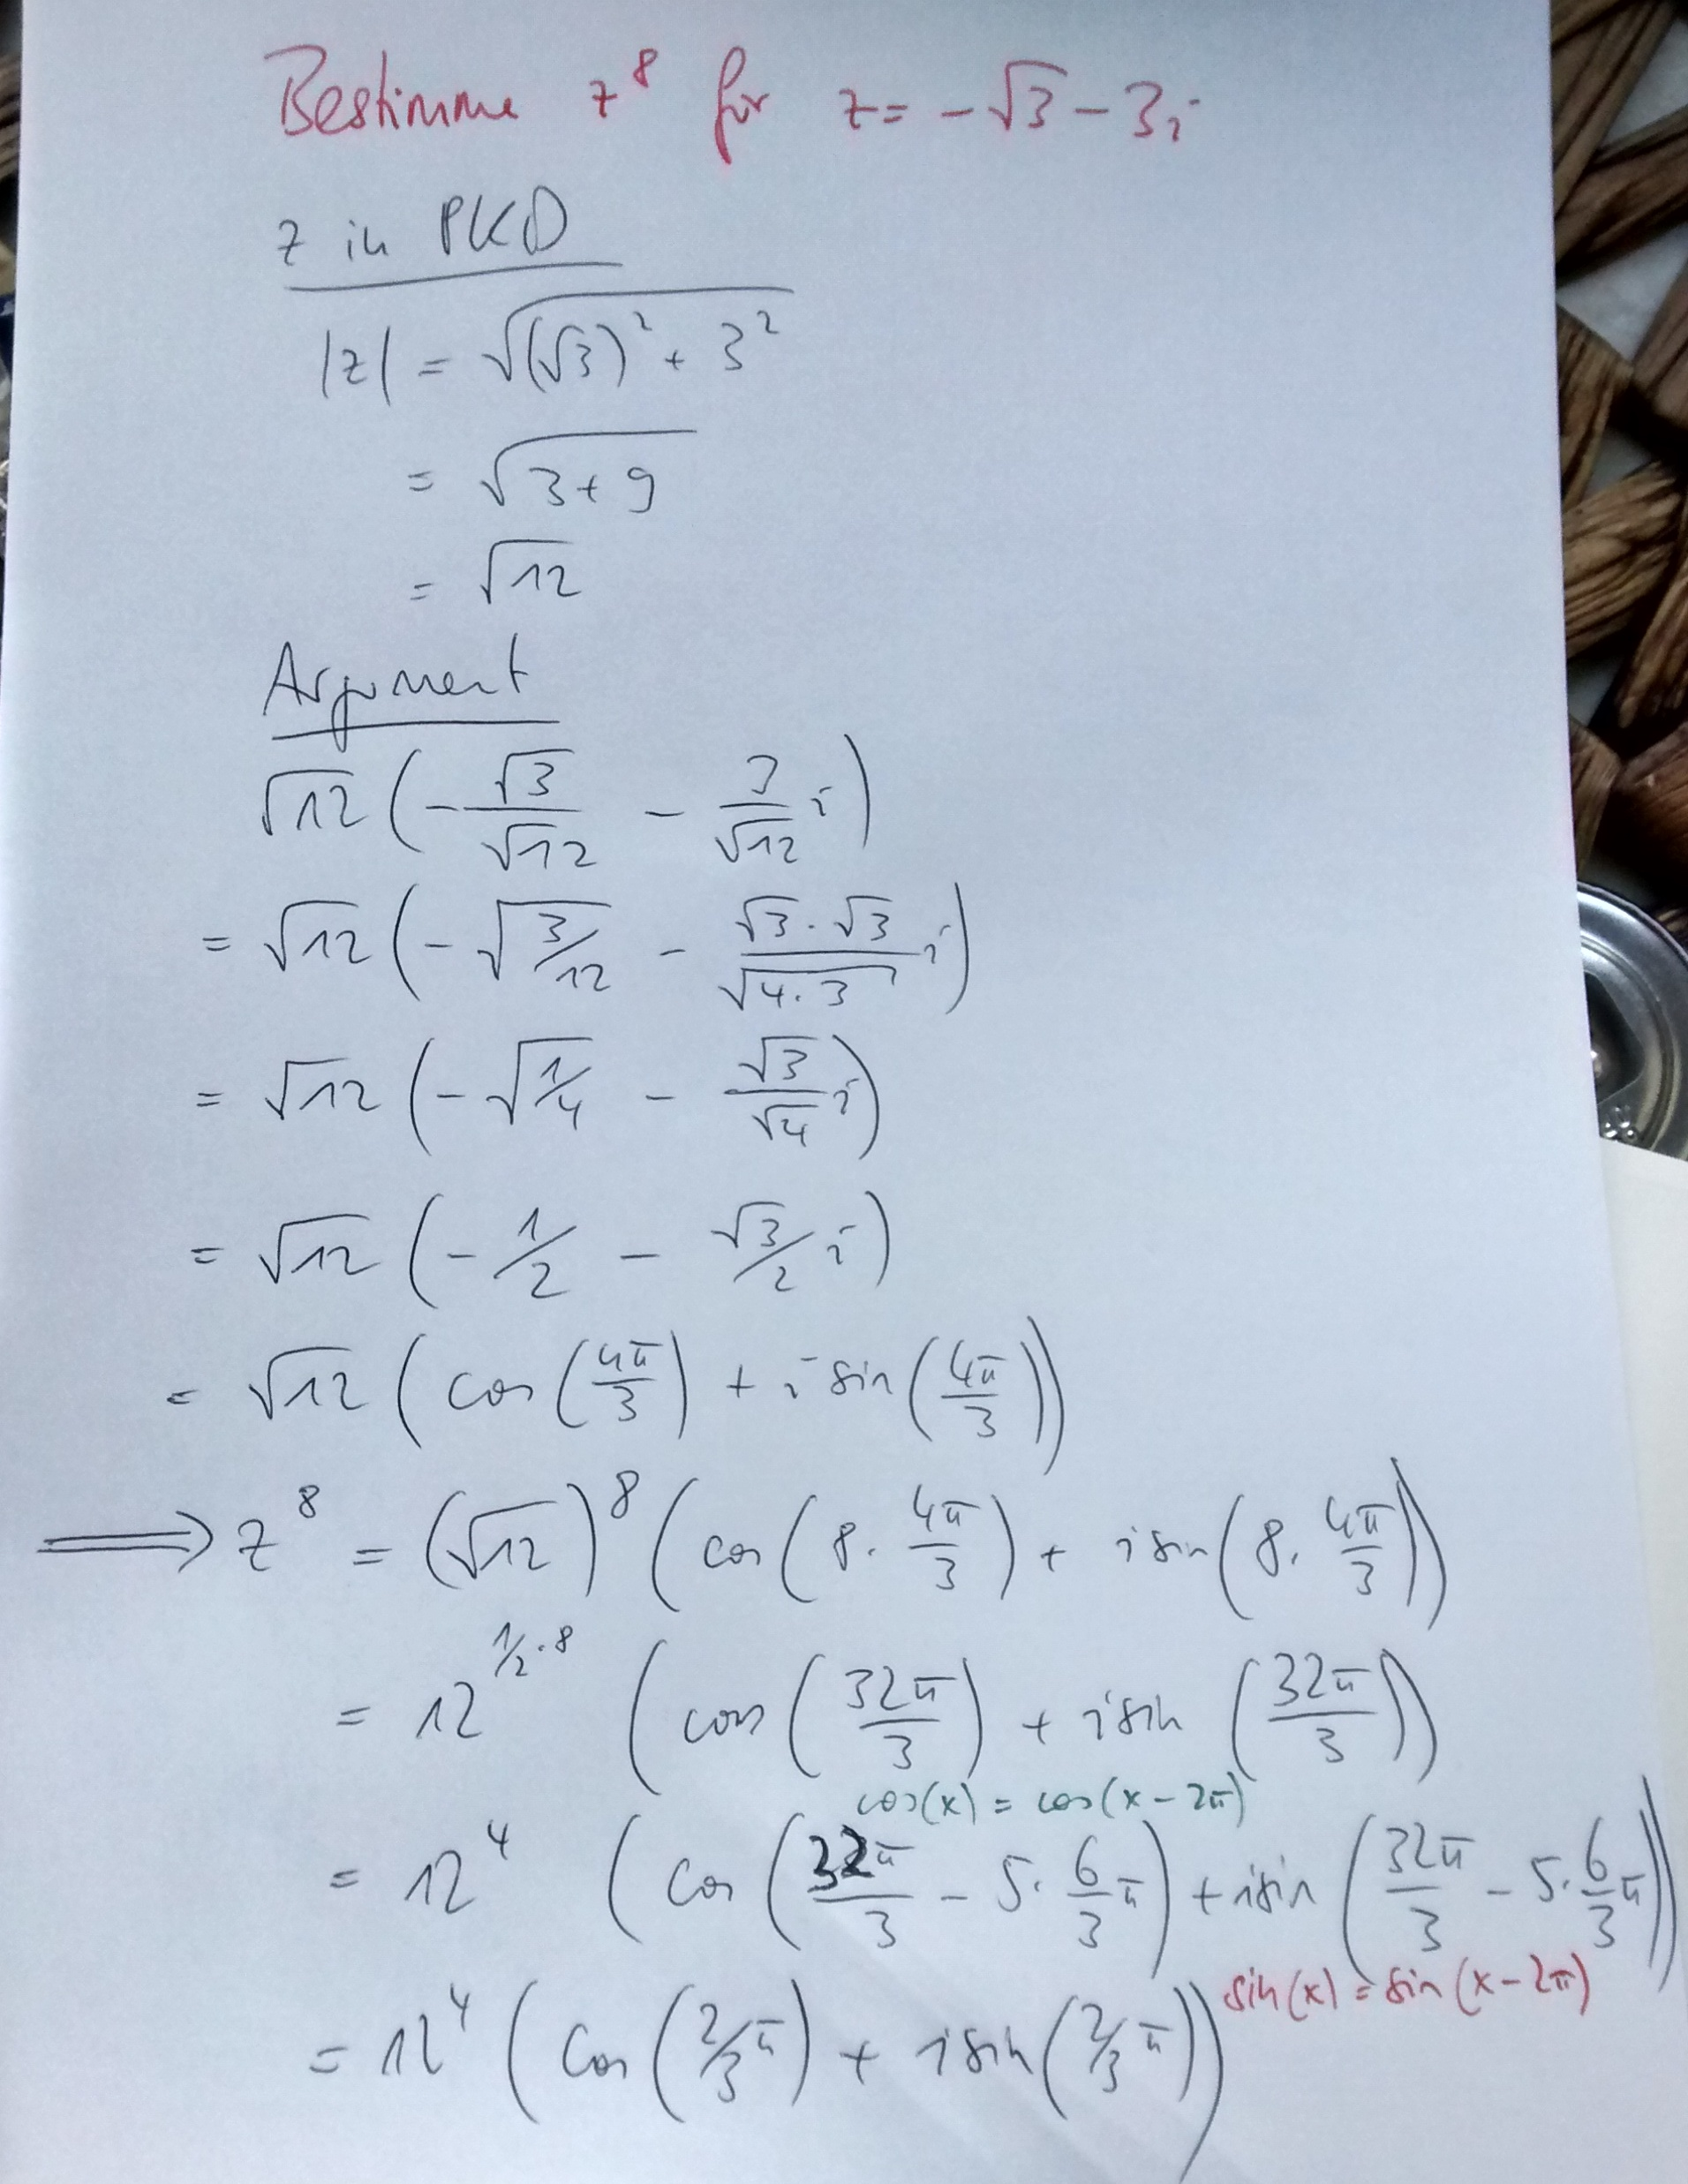
\includegraphics[width=1.0\textwidth]{img/testat_2_zhoch8.jpg}}
	\caption{Bestimmen von $z^8$}
	\label{fig:testat2_zhoch8}
\end{figure}


\newpage
\section*{Blatt 6}
\begin{itemize}
\item Wenn eine Zahl $z = x + iy \in \C$ in Polarkoordinatendarstellung (PKD) gebracht werden soll, reicht es nicht, nur den Betrag und den Winkel zu bestimmen. Es muss abschließend noch einmal $z$ in PKD angegeben werden. (Genauso wie am Ende immer noch einmal die Angabe der Gesamtlösungsmenge erwartet wird\dots)

\item Winkel werden in Bogenmaß gemessen (\texttt{RAD}). Winkel wie 360\textdegree, 180\textdegree, 90\textdegree, 60\textdegree~und 45\textdegree~sollte man in Bogenmaß kennen (oder sich eben schnell herleiten können).

Das Gradmaß (\texttt{DEG}) hat in der Mathematik nichts verloren (die Festlegung vom rechten Winkel auf 90\textdegree~ist recht willkürlich. Daneben (und auch deswegen) gibt es noch andere Gradmaße, mit denen man einfacher rechnen kann, z.\,B. \texttt{GON} mit mit einem rechten Winkel von 100~$\operatorname{gon}$)

\item Beim Umformen einer Zahl in PKD solltet ihr getrennt voneinander Winkel und Argument bestimmen (und dann noch einmal $z$ in PKD angeben, vgl.\,Abbildung~\ref{fig:testat2_zhoch8})


\item Bei der 1) b) ist $z_3$ \textbf{nicht} in PKD (man beachte das Minus vor dem Sinus). 

Soll hier mit $z_3$ gerechnet werden, muss das Minus zu einem Plus gemacht werden. 

Dieser Weg klappt immer: $z_3$ in die Form $x + iy$ bringen und dann in PKD umformen. Dann kann man die Rechengesetze für zwei komplexe Zahlen in PKD anwenden (z.\,B. das Rechengesetz für die Multiplikation). 

Geht evtl. schneller: Rechengesetze für $\sin$ und $\cos$ anwenden, um $z_3$ in PKD umzuformen. Achtung: \enquote{Beide} Winkel bei der PKD müssen gleich sein.

Solch eine Aufgabe ist auch auf einem der Trainingsblätter zu den komplexen Zahlen drauf. 

\item Wenn ihr im Argument von $\sin$ und $\cos$ rechnet, \textbf{setzt Klammern!} Sonst kann man nicht nachvollziehen, was ihr meint!
\begin{align*}
\cos \frac{3}{2}\pi - \pi 			&\stackrel{?}{=} 		\cos \left( \frac{3}{2}\pi - \pi  \right) \\
\cos \frac{3}{2}\pi - \pi 			&\stackrel{?}{=}			\cos \left( \frac{3}{2}\pi \right) - \pi 
\end{align*}

\item Für die PKD muss der Winkel aus $[0, 2\pi)$ sein. Das bedeutet insbesondere, dass der Winkel positiv angegeben wird! Sonst handelt es sich nicht um eine Zahl in PKD.

Ferner muss sowohl beim $\sin$ als auch beim $\cos$ \textbf{der gleiche Winkel} im Argument stehen.

\item Die Lösungen beim Wurzelziehen werden $z_0, z_1, \dots, z_{n-1}$ durchnummeriert. Dies sind die Lösungen der Gleichung
\begin{align*}
z^n = w
\end{align*}
mit $z, w \in \C$ und $w$ konkret. 

Eine Angabe von $z_n = z_0$ ist nicht erforderlich -- ich hatte das im Tutorium nur angeschrieben, damit ihr den zyklischen Aufbau versteht. 

\textbf{Tipp:} Zunächst Winkel getrennt von der Aufstellung der Lösungen berechnen. So macht ihr weniger Fehler.

Und gebt $w$ bitte einmal in PKD an, bevor ihr die Lösungen $z_0, z_1, \dots, z_{n-1}$ aufstellt. 


\item Standardwerte von $\sin$ und $\cos$ \textbf{muss} man auswendig wissen. Dazu zählen die Winkel $0, \frac{\pi}{2}$ und $\pi$. Es wird erwartet, dass diese Ausdrücke ausgewertet werden!

\item Macht ein ordentliches $\pi$! Bei einigen sieht das aus wie $n$, $\cap$ oder $\sqcap$.

\item Wenn ihr beim Sinus Klammern setzt, müsst ihr zwei Klammern schließen (die vom Sinus und die vom ausgeklammerten Betrag). Klingt bescheuert, vergessen aber 70\% von euch.

\item Rechnet \textbf{ohne} Taschenrechner. Rechnet mit Brüchen und Wurzeln usw. Tut euch den Gefallen!

\item Die Umkehrfunktion vom $\sin$ wird als Arcus-Sinus ($\arcsin$) bezeichnet. Sie liefert zu einer Zahl den Winkel (auf dem Taschenrechner ist das die Taste \texttt{sin\textasciicircum-1} -- auf das richtige Gradmaß im Taschenrechner achten! \dots aber den dürft ihr ja eh nicht benutzen \smiley{})

In der Mathematik wird die Schreibweise $\sin^{-1}(x)$ für den Arcus-Sinus nicht verwendet, weil man es nicht von $\frac{1}{\sin(x)}$ unterscheiden kann. Schreibt $\arcsin(x)$ für die Umkehrfunktion.

\item Wenn nicht weiter angegeben ist, wie die Lösung einer Rechnung angegeben werden soll, ist ein Ergebnis in PKD natürlich völlig in Ordnung.

\item Die \enquote{gemischte Bruchschreibweise} wird in der Mathematik nicht verwendet, da man nicht unterscheiden kann, ob $5\frac{1}{3}$ nun $5 \cdot \frac{1}{3}$ oder $5 + \frac{1}{3}$ bedeutet. 

\item Nach wie vor gilt: Gebt euch Mühe beim Setzen von Äquivalenz- und Gleichheitszeichen. Und setzt das richtige Zeichen an die richtige Stelle. Arbeitet mathematisch sauber! Sonst: Punktabzug!

Dazu: Wenn ihr das Zeichen $\stackrel{\wedge}{=}$ in der Mathematik verwendet, könnt ihr euch zu 90\% sicher sein, dass ihr es falsch oder unsauber notiert habt.

\item Es gilt: 
\begin{align*}
-64 \in \C.
\end{align*}
Überlegt euch, wie die PKD aussehen muss. Wo liegt die Zahl in der komplexen Ebene? 

\item Beim Bestimmen der PKD ist die Zahl, die ausgeklammert wird (also $|z|$), immer positiv. Dies muss insbesondere beim Bestimmen der PKD von $-64$ beachtet werden. 

Wenn ihr hier $64$ ausklammert, kommt ihr auf den richtigen Winkel von $\alpha = \pi$. 

Klammert ihr $-64$ aus, kommt ihr auf einen Winkel von $\alpha = 0$. Ein Winkel von $0$ hat aber keinen Sinn (überlegt euch, wo $-64$ in der komplexen Ebene liegt). 

\item Erinnerung: Die Vorschrift zum Bestimmen der Winkel für die Lösungen $z_1, z_2, \dots, z_{n-1}$ lautet (es sei $\varphi = \arg(z_k) = \frac{\arg(w)}{n}$ für $k = 0,1,2,\dots,n-1$):
\begin{align*}
\arg(z_k) = \varphi + k \cdot \frac{2\pi}{n} \qquad\text{für}\qquad k = 0,1,2,\dots,n-1
\end{align*}

\item Soll beim Wurzelziehen am Ende eine Lösungsmenge angegeben werden, reicht das aus:
\begin{align*}
\Lsg = \{z_1, z_2, \dots, z_{n-1}\}
\end{align*}

\item $2^5 = 32$, $2^6 = 64$. Zweierpotenzen bis $2^{10}$ sollte man auswendig wissen. 

\vfill

\item Maximal könnt ihr derzeit $20 + 19 + 4\cdot 5 = 59$ Punkte erreicht haben (Testate 1, 2) und (ÜB 2--6). Von insgesamt $20 \cdot 5 + 4 \cdot 13 = 152$ Punkten sind das 38\% und schon fast die Studienleistung, die es bei 60 Punkten gibt. Das heißt: Wer derzeit ca. 15 Punkte (25\% der Studienleistung) hat, \textbf{sollte Gas geben}! Es werden nur noch ca. 100 Punkte ausgeschüttet, von denen ihr dann 45 braucht! 

\end{itemize}









\newpage
\section*{Blatt 7}
\begin{itemize}
\item Kurzes Update: Es gilt lt. Skript $0 \in \R^{+}$ (Notation im Skript: $\R_{+}$).

\item Bei Polynomdivisionen \textbf{müssen} Klammern um den Dividenden gesetzt werden.\footnote{Dividend / Divisor = Quotient} Sonst wird nur das letzte (meist absolute) Glied durch den Divisor geteilt.

\item Kommt eine Nullstelle bei der $pq$-Formel oder sonstwo häufiger vor, taucht sie natürlich in der Linearfaktorzerlegung (LFZ) in entsprechender Potenz vor.

\item Wenn ihr die LFZ angeben sollt, gehört ein $f(x)$ vor die LFZ. Sonst steht der Rest einfach nur im leeren Raum. 

Also z.\,B.:
\begin{align*}
f(x) = -3(x-4)(x+5)(x-1)^7(x-1)^2
\end{align*}

\item Wenn ihr auf dem \enquote{Weg} zur LFZ z.\,B. bei einer Berechnung von der $pq$-Formel durch $2$ teilt (Aufgabe 1) a) iii)), dann dürft ihr die 2 nicht in der LFZ vergessen. Ihr hättet diese ja auch ganz (!) zu Beginn ausklammern können. Macht euch das klar.

\item \textbf{Beispiele sind keine Beweise!} Wenn in Aufgaben etwas wie \enquote{Zeigen Sie, dass \dots} steht, werden Beweise verlangt.\footnote{Die zu zeigende Behauptung stimmt -- im Gegensatz zu Formulierungen wie \enquote{Gilt \dots~für \dots} oder \enquote{Überprüfen Sie, ob \dots~gilt}, wo der Wahrheitsgehalt der Aussage gezeigt / widerlegt werden muss.} Für die Beweise lohnt sich ein Blick ins Skript.

\item Es gilt:
\begin{align*}
\frac{y}{2} = (x+1)^4\\
\Leftrightarrow \sqrt[4]{\frac{y}{2}} = |x + 1|
\end{align*}

Das ist etwas anderes als
\begin{align*}
\sqrt[4]{\frac{y}{2}} = x + 1.
\end{align*}

Siehe dazu auch die Musterlösung für weitere / die restlichen Umformungsschritte. 

\item Die Monotonie sollt ihr nicht über die 1. Ableitung zeigen. Das ist Stoff, der (noch nicht) behandelt wurde. Dies ist Stoff aus der  HM\RM{2}. Arbeitet deshalb mit der Definition im Skript. 

Dazu: $|x|$ ist in 0 nicht differenzierbar (diff'bar). $|x+3$ ist in $x = -3$ nicht diff'bar. Das heißt, man kann keine Ableitung in $x = 0$ bzw. $x = -3$ berechnen (u.\,a deswegen kann man die Monotonie nicht auf ganz $\R$ mit dem Ableitungskriterium zeigen). Das solltet ihr schon mal gehört haben; kommt ausführlich nächstes Semester.

\item Es gilt: $f(x) = |x|$ ist auf $\R$ weder (streng) monoton fallend noch (streng) monoton fallend. Ihr müsst die Funktion \textbf{als ganzes} und nicht nur ihre Äste sehen. Und den Definitionsbereich $\R$ beachten.

Dann tut eine Skizze ihr übriges:

\begin{figure}
\centering
\begin{tikzpicture}[domain=-4:4] 
    \draw[very thin,color=gray] (-3.9,-0.1) grid (3.9,3.9);
    \draw[<->] (-4.2,0) -- (4.2,0) node[right] {$x$}; 
    \draw[->] (0,-0.1) -- (0,4.2) node[above] {$f(x)$};
    \draw[color=red]    plot (\x,{abs(\x)})             node[right] {$f$}; 
\end{tikzpicture}
\end{figure}

\item Wenn man zu Beginn ein $x$ bei einem Polynom ausklammern kann, solltet ihr das tun. Dadurch werden Polynomdivision bzw.\,\textsc{Horner}-Schema kleiner. Macht euch das ggfs.\,klar.

\item Redet ihr von Funktionen, sprecht ihr diese natürlich beim Namen an. Auch wenn man überall immer $f(x)$ ließt, heißt die Funktion $f$. $f(x)$ bezieht sich auf die $y$-Werte (meist für ein oder mehrere \textbf{konkrete} $x$-Werte ($x = 7$, $x = -\pi$, \dots).

Es muss also korrekterweise heißen:
\begin{itemize}
\item $f$ ist streng monoton fallend (nicht $f(x)$)
\item $f$ ist stetig (nicht $f(x)$)
\item Der Graph von $f$ sieht aus wie \dots (nicht der Graph von $f(x)$)
\item $f$ ist differenzierbar (nicht $f(x)$)
\item $f$ ist bijektiv (nicht $f(x)$)
\item Es werden die Hoch- und Tiefpunkte von $f$ bestimmt (nicht von $f(x)$
\item $p$ hat den Grad 4 (nicht $p(x)$)\footnote{Ja, das habe ich letztes Tutorium beim Anschreiben selber nicht so angeschrieben -- mit Absicht. Ich glaube, es ist am Anfang einfacher, sich vorzustellen, dass $p(x)$ den Grad 4 hat, als dass $p$ den Grad 4 hat. $p(x)$ oder $q(x)$ erinnert mehr an ein Polynom als es vielleicht $p$ oder $q$ tut.}
\item usw. Es gibt vielfach mehr solche Beispiele.
\end{itemize}

\item Beim Zeigen von Gleichungen sucht ihr euch eine Seite aus und folgt dann durch einfache Termumformungen die andere Seite zu erhalten. Wenn $A = B$ zu zeigen ist, sehen die beiden Möglichen Lösungen so aus:
\begin{align*}
A = \dots = \dots = \dots = \dots = \dots = \dots = B
\end{align*}
oder
\begin{align*}
B = \dots = \dots = \dots = \dots = A
\end{align*}

Es kann sein, dass mal die Richtung von links nach rechts oder die von rechts nach links einfach ist als die jeweils andere. Da aber eben ein \enquote{$=$} dazwischen steht, sind beide Rechnungen gleichermaßen richtig.

\item Tipp für die Klausur: Aufgabenstellung lesen. Wer keine LFZ angibt, obwohl das in der Aufgabenstellung steht, kriegt Punktabzug. Auch wenn alle Nullstellen richtig sind und von mir aus auch ordentlich alle an einer Stelle angegeben werden. Gleiches gilt für die Angabe einer Lösungsmenge.

Zweiter Tipp: Lest jede Aufgabenstellung zwei mal. Und lest sie noch einmal, wenn ihr glaubt fertig zu sein, um zu checken, ob ihr nichts vergessen habt.

Dazu: Wenn nach Injektivität und Surjektivität gefragt ist, müsst ihr auch beides untersuchen.

\smiley{}

\item Die Aussagen
\begin{align*}
f \text{~surjektiv} \Rightarrow f \text{~nicht injektiv}
\end{align*}
oder 
\begin{align*}
f \text{~injektiv} \Rightarrow f \text{~nicht surjektiv}
\end{align*}
sind falsch. Injektivität und Surjektivität sind keine gegensätzlichen Begriffe und implizieren in keiner Weise einander.

Es gilt aber
\begin{align*}
\left(f \text{~nicht surjektiv} \lor f \text{~nicht injektiv}\right)   \Rightarrow f \text{~nicht bijektiv}.
\end{align*}

\item Es gilt im allgemeinen nur die Implikation 
\begin{align*}
f \text{~streng monoton} \Rightarrow f \text{~injektiv}.
\end{align*}
Die andere Richtung (Rückrichtung)
\begin{align*}
f \text{~streng monoton} \Rightarrow f \text{~injektiv}.
\end{align*}
ist falsch! Einige wollten damit die 3) a) ii) lösen. 

Ein Gegenbeispiel ist die Funktion $h \colon [0,2] \rightarrow [0,2]$ mit 
\begin{align*}
h(x) = \begin{cases}
-x+1 \quad  \text{für}\quad x \in [0,1)\\
x \quad \text{für} \quad  x \in [1,2]\\
\end{cases}
\end{align*}
Zeichnet euch die Funktion auf. $h$ ist injektiv (sogar bijektiv!), aber nicht streng monoton steigend oder steigend (auf $[0, 2]$ -- vgl.\,Überlegungen zur Betragsfunktion weiter oben). Das liegt daran, dass $h$ nicht stetig ist.

Ich habe das nicht so streng korrigiert, weil ihr die Stetigkeit der Funktion in der Aufgabe implizit vorausgesetzt habt (wenn anscheinend auch unbewusst\dots). Für stetige Funktionen gilt in obigen Implikationen nämlich $\Leftrightarrow$.

\end{itemize}




\newpage
\section*{Blatt 8}
\begin{itemize}
\item Wie bereits öfters erwähnt, wird die Angabe einer Lösungsmenge beim Lösen von Gleichungen verlangt. Und $Ax = b$ ist eine Gleichung.

\item Ihr dürft bei der 1) auch die Schritte a)--d) für jedes LGS zusammen machen. Dann bleibt man in der Aufgabe.

\item \textbf{Schreibt beim Umformen eines LGS daneben, was ihr rechnet bzw. welche Zeile ihr \emph{wie} manipuliert.} Die Notation sollte wie im Tutorium besprochen erfolgen. 

\item Ihr solltet für Parameter $s$ und $t$ schreiben und nicht die Variable nutzen. Das heißt, ihr gewinnt aus einer Zeile die Information, dass  $x_3$ beliebig ist, und solltet dann $x_3 =: t$ notieren (und mit $t$ für $x_3$ weiter rechnen).

\item Die Lösungsmenge wird bei $\infty$-vielen Lösungen wie im Tutorium wie folgt angegeben. Ihr geht vom groben (erst alle Vektoren $x \in \R^3$) ins Feine ($x$ soll solche Gestalt haben: \dots -- das bedeutet der Strich \enquote{$\mid$}). Eine andere Richtung ist nicht sinnvoll.
\begin{align}
\Lsg = \left\{ x \in \R^3 \mid x = \Spvek[c]{1;1;0} + t\Spvek[c]{-1;1;1}, t \in \R\right\} \label{eq:lsg_axb_infty}. 
\end{align}

Ihr solltet die Vektoren, falls es $\infty$-viele Lösungen gibt, trennen (so wie in der Lösungsmenge (\ref{eq:lsg_axb_infty}) oben). Dann erkennt man besser, welche die Lösung (Singular!) des inhomogenen $Ax = b$ und welches die Lösungen (Plural!) des homogenen Systems $Ax = 0$ sind (den genauen Zusammenhang beider Systeme werden wir wahrscheinlich noch mal im Tutorium besprechen).

Ist nur \emph{ein} Vektor in der Lösungsmenge, kann dieser einfach angegeben werden, z.\,B.:
\begin{align*}
\Lsg = \left\{\Spvek[c]{\frac{1}{7};1;-2}\right\}. 
\end{align*}

Nicht die Klammern um den Vektor vergessen! 

Angaben wie 
\begin{align*}
\Lsg = \left\{x = \frac{1}{7}, y = 1, z = -2\right\} 
\end{align*}
sind nicht wirklich sinnvoll, weil nur ein \textbf{Vektor} das LGS $Ax = b$ löst.

 
Und es heißt $\Lsg = \{\dots\}$, nicht $\Lsg : \{\dots\}$
\item Wenn etwas wie \enquote{Ist $v \in \Lsg$?} gefragt ist, wird auch ein Antwortsatz erwartet. Ich habe dann \enquote{Aussage?} daneben geschrieben.

\item Der Vektor in 2) b) ii) heißt $v$. $v^\intercal$ ist nur eine verkürzte Schreibweise eines Spaltenvektors als Zeile (damit das im Text nicht so viel Platz weg nimmt). 

Also: Es wird überprüft, ob $v$ in $\Lsg$ ist, nicht ob $v^\intercal \in \Lsg$ gilt.

\item Fallen bei der Vorwärtselimination Zeilen raus (weil sie identisch sind), schreibt für diese Zeile $0 = 0$ und lasst diese nicht einfach weg.\footnote{Das Weglassen wäre mathematisch nicht falsch, es ist aber leichter für die Korrektur, wenn die Zeilen stehen bleiben. Und es sieht nicht wie ein \enquote{neues} System aus. \smiley{}} 

Beispiel:
\begin{align*}
\left(
\begin{array}{ccc|c}
1 & 3 & 4 & 1\\
1 & 5 & 7 & 1\\
1 & 3 & 4 & 1\\
\end{array}
\right)
&
\Leftrightarrow
\left(
\begin{array}{ccc|c}
1 & 3 & 4 & 1\\
  & 2 & 3 & 0\\
  &   & 0 & 0\\
\end{array}
\right)
\end{align*}
Eher nicht (s.\, Fußnote): 
\begin{align*}
\left(
\begin{array}{ccc|c}
1 & 3 & 4 & 1\\
1 & 5 & 7 & 1\\
1 & 3 & 4 & 1\\
\end{array}
\right)
&
\Leftrightarrow
\left(
\begin{array}{ccc|c}
1 & 3 & 4 & 1\\
  & 2 & 3 & 0\\
\end{array}
\right)
\end{align*}

\item Zwischen die Umformungsschritte bei der Vorwärtselimination gehört ein \enquote{$\Leftrightarrow$} oder \enquote{$\rightsquigarrow$}. Ganz bestimmt aber nicht \enquote{$=$}, weil die Schreibweise $\left(A|b\right)$ ja schon eine verkürzende Schreibweise für Gleichungen ist. 

\item Es gibt mehrere Wege, die nach Rom führen (bzw\,zur ZSF) \smiley{}

Wenn die ZSF angegeben werden soll (Aufgabe 1), solltet ihr das auch tun. Auch im Hinblick auf die (Probe-)klausur.

Die Matrix
\begin{align*}
\left(
\begin{array}{ccc|c}
1 & 3 & 4 & 1\\
1 & 0 & 0 & 8\\
0 & 3 & 4 & 4\\
\end{array}
\right)
\end{align*}
ist nicht in ZSF (auch wenn man die Lösungsmenge sehr leicht bestimmen kann: \RM{2}~$\rightarrow$~\RM{3}~$\rightarrow$~\RM{1}).

\item Nur, dass ich es mal erwähnt habe:
\begin{align*}
\Spvek[c]{0;1;-2;-5} \in \R^4 \qquad \Spvek[c]{0;1;-2;-5;9} \in \R^5
\end{align*}

\item $\operatorname{rang}(A) > \operatorname{rang}(A|b)$ ist nicht möglich (klar machen!). Notation ist wie folgt: $\operatorname{rang}(A) = 3$, nicht $\operatorname{rang}(A) : 3$.

\item Macht Klammern um Matrizen (und Vektoren sowieso)! Eckige Klammern um Matrizen werden hauptsächlich im englischsprachigen Raum (und der Numerik) verwendet; wir verwenden runde klammern.

\item Ihr dürft Vektoren nur mit Zahlen $\gamma \in \R$ multiplizieren. Die Division ist in den Vektorraum-Axiomen für Skalare nicht definiert und ihr müsst sie über eine Multiplikation mit $\frac{1}{\gamma}$ ausdrücken. Das heißt:
\begin{align*}
\qquad\text{erlaubt:}\qquad\frac{1}{7}\Spvek[c]{-5;38;-5} =  \Spvek[c]{-\frac{5}{7};\frac{38}{7};-\frac{5}{7}}; \qquad\text{nicht erlaubt:}\qquad \Spvek[c]{-5;38;-5} : 7
\end{align*}
\end{itemize}

\vspace{1cm}

\begin{center}
\fontsize{18pt}{18pt}{{\calligra Fröhliche Weihnachten und einen guten Rutsch!}}
\end{center}








\newpage
\section*{Probeklausur Dezember 2016}
\subsection*{Aufgabe 1}
\begin{itemize}
\item[a)] \textbf{Trick} 3. binomische Formel im Zähler ausrechnen. 

Und aufpassen: $\frac{1}{2}(1 + 3i)$ ist \textbf{nicht} in der Form $a+ ib$. Punktabzug (Aufgabenblatt!).

\item[b)] Auf den richtigen Winkel achten (Quadrant!). Es muss erkennbar sein, dass die Winkeltabelle benutzt wurde (Aufgabenblatt). 

\enquote{Beide Winkel} müssen in der PKD gleich sein.

\item[c)] \textbf{Tipp} Skizze machen, wo die Zahl $z = 8$ liegt. Dann kann der Winkel abgelesen werden (Winkel $\alpha = \pi$ ist falsch!).

$\sqrt[3]{8} = 2$ muss ausgerechnet werden (sollte man wissen).

Standardwerte von Sinus und Cosinus müssen ausgewertet werden. Insbesondere $\sin(0)$, $\cos(0)$, $\sin(2\pi)$, $\cos(2\pi)$.

\item[d)] Von der einen Seite zur anderen beweisen. Dabei das $k$ im Zähler mit dem $k!$ im Nenner kürzen (Fakultäten ausnutzen!). 

Es gilt $(n - k)! = (n - 1 - k + 1) =  (n - 1 - (k - 1))$. Das sieht man, wenn man weiß, \enquote{wo man hin will}.

Die Beweisrichtung von rechts nach links geht auch. 

Ausschließliches Umschreiben des Binomialkoeffizienten gibt keine Punkte.

\item[e)] \textbf{Trick} Bei der i) muss ein $1^k$ ergänzt werden, um den binomischen Lehrsatz anwenden zu können. Dann erhält man $(1+i)^8$. Mit dem Hinweis, dass das Ergebnis reell sein soll, rechnet man wie folgt (schneller als \textsc{DeMoivre} und weniger fehleranfällig). 
\begin{align*}
(1+i)^8 = \left((1+i)^2\right)^4 = (2i)^4 = 2^4 \cdot i^4 = 16 \cdot \left(i^2\right)^2 = 16 \cdot (-1)^2 = 16 \cdot 1 = 16
\end{align*}

Die Lösung $(1+i)^8$ ist nicht ausreichend (s. Aufgabenblatt).

\textbf{Trick} Bei der ii) keine Indextransformation machen. Das macht den Binomialkoeffizienten unschön. Guckt man sich an, was $x$ und $y$ sind, so stellt man fest, dass $x + y = -2 + 2 = 0$ ist. Es ist also sinnvoller, den bin. Lehrsatz für $k=0$ bis $k = 11$ anzuwenden (es ergibt sich $0$) und dann den Summanden, den man zu viel gezählt hat (es ist der Summand für $k = 0$) vom Ergebnis abzuziehen. Man erhält dann $0 - (-2)^{11} = 2048$.

\item[f)] Aufpassen! Wenn ihr vergesst, einen $x$-Wert zu überprüfen, gibt es Punktabzug. Es müssen minimal drei Fälle untersucht werden (Betrag führt zu zwei Fällen und die Ungleichung -- durch das $x$ im Nenner --  auch zu zweien. Diese können in drei Fällen zusammengefasst werden). Eine Tabelle hilft dabei. 

Definitionslücke bei $x = -1$ beachten. Ein Fall wie $x < 1$ ist zu grob (was ist mit $x = -1$?).

Auch wichtig: Lösungsmengen für die einzelnen Fälle angeben! Und die Gesamtlösungsmenge $\Lsg_{\text{Ges}}$ angeben (richtig vereinigen -- sonst Punktabzug, s. Anmerkungen bei dem entsprechenden Blatt weiter oben).

\item[g)] Matrix in ZSF bringen und Rückwärts einsetzten. Wird keine Lösungsmenge angegeben, gibt es keinen Punkt für die Lösung (Aufgabenblatt!). 

Ob der Vektor $x \in \Lsg$ ist, kann auch unabhängig vom Rest der Aufgabe beantwortet werden (nachrechnen, vergleiche auch den Lösungsvorschlag zum 3. Testat).
\end{itemize}

\subsection*{Aufgabe 2}
\begin{itemize}
\item[a)] Beim (IA) darf in der Summe nicht sofort das $k$ durch $2$ ersetzt sein (siehe Anmerkungen zum entsprechenden Übungsblatt oben). Punktabzug.

Sollte der (IA) schief gehen, ist der \enquote{Beweisversuch} (der Induktionsschritt) überflüssig. Die Induktion baut insbesondere auf dem (IA) auf (Induktionsprinzip).

Rechenregeln der Fakultät beachten (typische Fehler sind weiter oben schon diskutiert). 

\textbf{Trick} Die beiden Summen nach Einsetzten der (IV) nicht auf einen Hauptnenner bringen, sondern den Summanden, in dem $n!$ im Nenner steht, mit $(n+1)$ erweitern, sodass beide Nenner gleich sind (Es gilt: $n! \cdot (n+1) = (n+1)!$ -- klar machen, warum das gilt!).

\item[b)] \textbf{Trick} $z\overline{z} = |z|^2$ und $-z+\overline{z} = -2\text{Im}(z)$. Das macht es zu Beginn einfacher. 

Zum Bestimmen von Real- und Imaginärteil der Lösung einen Koeffizientenvergleich machen.

Vorsicht: Nicht die Lösung $a = -3$ vergessen bei $a = \sqrt{9}$. Sonst Punktabzug.

Auch hier muss eine Lösungsmenge angegeben werden.

\item[c)] Es müssen (in der Regel) beide Additionstheoreme verwendet werden, die auch auf dem Aufgabenblatt angegeben wurden.

\item[d)] Polynomdivision machen. Daran kommt man nicht vorbei. Dabei stellt man fest, dass diese auf geht und man wirklich den Linearfaktor ohne Rest abspalten kann. Daher weiß man, dass $n_1 := 2i - 1$ eine Nullstelle ist.

\textbf{Trick} Da $f$ nur Koeffizienten aus $\R$ hat, ist $n_2 := \overline{n_1} = -2i - 1$ auch eine Nullstelle (wurde im Tutorium besprochen).

Dann kann man diese mit dem \textsc{Horner}-Schema abspalten (geht wahrscheinlich schneller als die Division $f(z) : ((z - n_1)(z - n_2))$ und man erhält die dritte Nullstelle: $n_3 := -3$. Man kann dann die LFZ angeben. 

Für die Kontrolle: Da $3\cdot(-1-2i)\cdot(-1+2i) = 15$ gilt, ist kein  Vorfaktor bei der LFZ nötig.

\item[e)] Nur am Bild zu argumentieren reicht nicht. Rechnerisch lösen! Das meint nicht, dass man konkrete Zahlen einsetzt und dann guckt, ob es injektiv oder surjektiv ist. Das sind nur Beispiele und keine Beweise.

Achtung: Geraden sind nicht automatisch surjektiv oder injektiv. Was ist zum Beispiel mit einer Parallelen zur $x$-Achse?

Aufgabenstellung lesen: Wenn $f$ bijektiv ist, soll eine Umkehrabbildung angegeben werden. Fehlt diese, gibt es natürlich Punktabzug.

\item[f)] Gesucht war hier:
\begin{itemize}
\item Menge, die nur den Nullvektor $0_{\R^3}$ enthält
\item Gerade \textbf{durch den Nullpunkt}
\item Ebene \textbf{durch den Nullpunkt}
\item $\R^3$
\end{itemize}

Klar machen, warum das UVR von $\R^3$ sind. Geraden und Ebenen, die nicht durch den Nullpunkt gehen, sind keine UVR (es sollte jeder begründen können, wieso dies so ist).

Weiterführende interessante Fragestellung: Wie sehen alle Typen von UVR im $\R^2$ oder $\R^5$ aus?
\end{itemize}







\newpage
\section*{Testat 3}
\begin{itemize}
\item Beim LGS kann man auch anders herum die richtige Lösung finden, indem man sich fragt, ob der Ortsvektor der Hyperebene der Lösungsmenge (die Lösungsmenge ist eine Hyperebene im $\R^6$) das LGS löst (Matrix-Vektor-Multiplikation). Dies hatte ich ja auch in den Tutorien schon einmal erwähnt.

\textbf{Tipp} Ansonsten die Variablen frei wählen, bei der keine Stufe in der ZSF ist. Das heißt, wenn zwei Variablen $x_k$ und $x_j$ frei gewählt werden können, wählt diejenige als frei, bei der der Index \textbf{größer} ist. Das haben wir bisher immer so gemacht (s. Tutorium) und es ist einfacher zu korrigieren (auch wenn das andere auch richtig ist). Falls ihr anders vorgeht, werdet ihr eure Lösung evtl. nicht unter den Lösungsvorschlägen gefunden haben, auch wenn eure Lösung richtig war (klar machen, warum es \enquote{verschiedene} Lösungen gibt. Das heißt, obwohl die Lösungsmengen eigentlich verschieden aussehen, sind sie doch identisch).

Das LGS ist bereits in ZSF. 

\item Bei der Polynomdivision können Ergebnisse mit einem Koeffizienten $\neq 1$ vor dem $z^2$ direkt ausgeschlossen werden. Klar machen, warum dies geht.

\item Bei den Funktionen geht es am schnellsten, die Frage nach Injektivität, Surjektivität und Bijektivität mit einer Zeichnung zu entscheiden. Wo schneiden Parallelen zur $x$-Achse den Graphen von $f$ nicht / einmal / mehrmals / genau einmal? (Auf den Wertebereich achten! -- nur dort dürfen Parallelen gezogen werden).
\end{itemize}














\newpage
\section*{Blatt 9}
\begin{itemize}
\item In der 1) b) i) soll die Mengendefinition des Spanns angegeben werden. Nur die Vektoren als Spann aufzuschreiben ist nicht ausreichend.

Zu sagen, dass der Spann ein Erzeugendensystem ist, ist falsch. Nur Vektoren können ein EZS bilden. Und ihr müsst sagen, welcher Raum erzeugt wird. Ohne diese Angabe ist das wie die Aussage: \enquote{Die Zahl $9$ ist größer.} ($\rightarrow$ Größer als was?)

Ohne Rechnung oder Begründung kann man nicht sagen, dass die Vektoren den $\R^3$ erzeugen. Das \enquote{sieht} man hier auch nicht. 

\item Zur ii): \enquote{anschaulich} meint hier die Argumentation, dass vier Vektoren im $\R^3$ immer (!) linear abhängig sein müssen. Das hat Dimensionsgründe, die man sich leicht überlegen kann.

Die Lineare Abhängigkeit / Unabhängigkeit von Vektoren kann man an der Matrix in ZSF ablesen.

\item Zur iii): Mit der anschaulichen Argumentation aus ii) ist dann auch klar, dass die Vektoren keine Basis des $\R^3$ bilden können. 

Werden schon senkrechte Vektoren ausgewählt, ist die ONB mit \textsc{Gram-Schmidt} in iv) leichter zu berechnen.

Hinweis dazu: Vor dem normieren könnt ihr Vektoren natürlich vereinfachen. Ist in jeder Komponente des Vektors bspw. ein $\frac{1}{9}$ vorhanden, könnt ihr die $\frac{1}{9}$ ausklammern und unter den Tisch fallen lassen (Vorsicht beim Aufschrieb: Die Vektoren sind natürlich nicht gleich! Sie zeigen nur in die gleiche Richtung!) Dann muss nur noch der Vektor mit den ganzen Zahlen normiert werden.

\item Zur v): Die einfachste ONB ist hier natürlich $e_1, e_2, e_3$. Man sieht auf Anhieb, dass die Vektoren die Länge $1$ haben und paarweise senkrecht stehen.

\item Basen werden ohne Mengenklammern angegeben. Schreibt einfach: Basis von $\R^3$: $v_1$, $v_2$, $v_3$.

\item Der Spann von Vektoren ist keine Basis! Der Spann ist zunächst eine Menge. Zudem enthält der Spann unendlich viele linear abhängige Vektoren (der Spann enthält immer unendlich viele Vektoren!). 

Dass der Spann immer ein Unterraum ist, ist keine Begründung dafür, dass der Spann eine Basis \emph{sei}. Es ist eine Begründung dafür, dass der Spann generell eine Basis \emph{hat}. 

Es gibt nicht \emph{die} Basis eines Vektorraums. Es gibt (von einigen Spezialfällen mal abgesehen\footnote{Überlegt mal, welchen Spezialfall ich meine. Einen haben wir kennengelernt. Spontan fällt mir auch kein zweiter ein\dots \smiley{}}) unendlich viele verschiedene Basen eines Vektorraums. Alle Basen haben aber dieselbe Länge.

\item Für eine ONB müssen \textbf{alle} Basisvektoren paarweise senkrecht stehen und normiert sein.

\item Die Norm eines Vektors wird mit $\|v\|$ notiert. Die Norm ist gewissermaßen die Weiterführung des Betrags (also $|x|$) aus den reellen Zahlen in die höherdimensionalen Räume und beschreibt die Länge des Vektors (also die Länge des Vektorpfeils).

\item Zur c): Ihr könnt natürlich vorher überprüfen, welche Vektoren linear abhängig sind, sodass ihr für diese gar nicht erst \textsc{Gram-Schmidt} machen müsst.

Steckt ihr einen linear abhängigen Vektor in das \textsc{Gram-Schmidt}-Verfahren, kommt am Ende der Nullvektor heraus. Dieser ist per Definition linear abhängig und wird nicht zur Basis gezählt.

Generell ist es aus Dimensionsgründen nicht sinnvoll, im $\R^4$ \textsc{Gram-Schmidt} für $5$ Vektoren zu machen. Dies ist anschaulich klar (vgl. Aufgabe b) ii)). Eine Basis im $\R^4$ besteht natürlich aus $4$ Vektoren. Da braucht man nicht einen 5. Vektor für die Basis zu bestimmen (diesen gibt es auch gar nicht!). Das Problem könnt ihr euch im $\R^2$ auch gut aufzeichnen. Ihr findet keinen dritten Vektor, der zu $(1, 0)^\intercal$ \textbf{und} $(0, 1)^\intercal$ orthogonal ist.

\item Für die c) ii) muss man natürlich kein LGS lösen, sondern kann die Koeffizienten leicht mit der Formel aus dem Skript bestimmen (s. Testat 4 unten).

\item Das Skalarprodukt zweiter Vektoren ist eine reelle Zahl!

\item Zur 2) a): Soll hier nachgewiesen werden, dass es sich um einen Untervektorraum handelt, solltet ihr angeben, was der Oberraum ist. Dies ist hier der $\C^{2 \times 2}$ bzw. $\C^{3 \times 3}$.

Die Mengen dürft ihr natürlich benennen. Mengen werden mit Großbuchstaben benannt, Vektoren mit kleinen Buchstaben.

Auch wenn die Mengen Matrizen enthalten, spricht man von Vektoren. Es heißt ja \emph{Vektor}raum.

Als Tipp kann man festhalten: Immer wenn irgendwelche Komponenten für einen UVR so verrechnet werden sollen, dass eine Zahl $\neq 0$ dabei herauskommen soll, handelt es sich in der Regel nicht um einen UVR (weil immer das UVR-Axiom \RM{2} nicht erfüllt ist).

Das Nullelement, also das neutrale Element der Addition, ist hier die Nullmatrix. Ihr könnt diese als $0_{\C^{2 \times 2}}$ bezeichnen, um sie von der $0_\R$ zu unterscheiden.

Nach wie vor gilt: Beispiele sind keine Beweise! Beispiele sind nur erlaubt, sollen Aussagen widerlegt werden.

\item Die Matrix aus c) i) ist überhaupt kein Element der beschriebenen Menge. Sie kann also auch nicht dargestellt werden. Ihr solltet zu Beginn immer überprüfen, ob der darzustellende Vektor überhaupt Teil der Menge ist. 

\item Für die Darstellung der Matrix aus c) ii) muss man sich natürlich vorher eine Basis überlegen. Die Basis besteht aus drei Vektoren (Vektoren sind hier Matrizen, wie schon erwähnt).

Ihr solltet euch überlegen, warum es ausreicht, dass die Matrizen der Basis immer nur Einsen und Nullen enthalten (Stichwort $\C$-Vektorraum). Welche Vektoren müsste die Basis enthalten, wenn die Menge als $\R$-Vektorraum und als Teilmenge von $\C^{2 \times 2}$ aufgefasst werden würde?

\item Zur Aufgabe 3: Generell gilt: $\text{dim~} \Poly_n = n + 1$, also $\text{dim~} \Poly_2 = 3$.

\item Zur a) i): Gebt an, wie ihr die Koeffizienten berechnet (habt). Ihr könnt zur Lösung die Aufgabe auch in Matrizenschreibweise umformen. Wenn ich das Gefühl hatte, dass ihr nicht wisst, wie die Darstellung funktioniert, habe ich das nicht durchgehen lassen (und \enquote{woher?} dran geschrieben). 

\item Zur ii): Soll die lineare Unabhängigkeit gezeigt werden, geschieht dies am einfachsten über die Definition der linearen Unabhängigkeit.

\item Zur iii) Die Vektoren $p_1$ und $p_2$ können allein aus Dimensionsgründen keine Basis von $\Poly_2$ sein (selbes Argument wie in b) ii) nur anders herum).

Wenn berechnet wurde, dass der Vektor $q(x) = x^2 + x + 1$ nicht mit $p_1$ und $p_2$ dargestellt werden kann (und das $p_1$ und $p_2$ deshalb keine Basis bilden können), ist das natürlich auch in Ordnung. Eine Basis muss nämlich jeden Vektor des Raums erreichen können.

\item Die Vektoren (hier Polynome) heißen $p_1$, $p_2$ (und nicht $p_1(x)$ oder $p_2(x)$ -- siehe oben).
\end{itemize}







\newpage
\section*{Testat 4}
\begin{itemize}
\item Wenn ihr das LGS in 1) gelöst habt, ist die 2) geschenkt. Es ist für 2) genau dasselbe LGS zu lösen. Die Koeffizienten $\lambda_1, \lambda_2, \lambda_3$ habt ihr dann schon berechnet.

Die meisten Fehler in der 1) bestanden daraus, dass die Lösungsmenge $\Lsg$ nicht korrekt aufgeschrieben wurde. Das solltet ihr mittlerweile beherrschen, da das zur Genüge in den Globalübungen, Tutorien und VL gemacht wurde. Da Punkte zu verlieren ist extrem ärgerlich. Und das habe ich hier auch aufgenommen (siehe oben).

\item In der 3) löst man natürlich kein LGS, sondern verwendet die Formel für die Koeffizienten, wenn man eine \textbf{ONB} gegeben hat (Achtung: Das geht natürlich nur bei einer ONB!). Diese Formel lautet:
\begin{align*}
\mu_i = \langle w, u_i \rangle,
\end{align*}
wobei $\langle \cdot, \cdot \rangle$ das Skalarprodukt meint ($w$ soll dargestellt werden, $u_i$ ist der $i$-te Basisvektor der ONB).

\end{itemize}





\newpage
\section*{Blatt 10}
\begin{itemize}
\item Für die Linearität müssen beide Eigenschaften gezeigt werden. Das ist die Linearität unter der Addition (L1) und die Linearität unter skalarer Multiplikation (L2).

Der Schluss
\begin{align*}
f(0) = 0 \Rightarrow f \text{~linear}
\end{align*}
ist falsch. Die Forderung ist zu schwach. Zum Beispiel gilt $\sqrt{0} = 0$, aber die Wurzelfunktion ist nicht linear (kann man sich leicht überlegen!).

Es gilt nur 
\begin{align*}
f(0) \neq 0 \Rightarrow f \text{~nicht~linear}
\end{align*}

\textbf{Achtung!} Im Argument von $f$ werden Vektoren \textbf{als Zeilen} geschrieben! Das heißt, wir schreiben
\begin{align*}
f(x+a,y+b,z+c) 
\end{align*}
und nicht
\begin{align*}
f\left(\Spvek[c]{x;y;z} + \Spvek[c]{a;b;c}\right).
\end{align*}

Das Nachrechnen der Linearität von Abbildungen erfolgt wie im Tutorium. 

\item Die Aufgaben 1) b) und c) gehören sicherlich zu den interessanten Aufgaben auf dem Blatt. Diese sind besonders wichtig.

\item Die Matrix kann nur eine $3 \times 3$-Matrix sein, weil sonst keine Abbildung von $\R^3$ nach $\R^3$ vorliegt.

Da die Basis des Bildes vorgegeben ist und die linear unabhängigen Spaltenvektoren von $A$ immer eine Basis des Bildes bilden, kann für den dritten Spaltenvektor von $A$ ein linear abhängiger Vektor gewählt werden. Dieser liegt im Spann der anderen beiden (klar) und sowieso im Bild (damit auch klar). Im einfachsten Fall wählt man
\begin{align*}
a_3 = \Spvek[c]{0;0;0}.
\end{align*}

\item Zur c): Man überlegt sich zunächst, dass die Matrix eine $3 \times 4$-Matrix sein muss. Da $\dim \text{Kern} f = 2$ nach der Aufgabenstellung gilt, braucht die Matrix nach dem Dimensionssatz zwei linear unabhängige Spalten bzw. Zeilen (Zeilenrang = Spaltenrang; Argumentation über das Bild).

Als Ansatz wählt man dann  

\begin{align*}
A = 
\left(
\begin{array}{cccc}
1 & 0 & a & b\\
0 & 1 & c & d\\
0 & 0 & 0 & 0\\
\end{array}
\right).
\end{align*}

Dann erhält man über die Rechnungen 
\begin{align*}
A\cdot v_1 = 0 = 0_{\R^3}
\end{align*}
und
\begin{align*}
A\cdot v_2 = 0 = 0_{\R^3}
\end{align*}
ein LGS, das man dann für $a$, $b$, $c$ und $d$ lösen kann. Weiteres wird in der Globalübung / Musterlösung erklärt.

\textbf{Vorsicht} Viele hatten 
\begin{align*}
A\cdot v_i = 0 = 0_{\R^4}
\end{align*}
gerechnet, aber das ist natürlich falsch (so funktioniert die Matrixmultiplikation nicht).

\item Sollen $2 \times 2$-Matrizen invertiert werden, geht dies schneller über die Formel als mit \textsc{Gauß}.

\item Vorsicht bei der Multiplikation von Matrizen und dem Transponieren von Produkten:
\begin{align*}
(AB)^\intercal = B^\intercal A^\intercal
\end{align*}

Solche Regeln gelten auch beim Invertieren! Vorsicht!

\item Für die Aufgabe 2) b): $D^{-1}$ kann auch über die Adjunkte Matrix bestimmt werden (siehe Skript).

\item Aufgabe 3) b) ist auch interessant. 

\textbf{Achtung!} Auf dem Blatt war ein Tippfehler. Die Abbildung muss von $\R^4$ nach $\R^3$ gehen (sonst passt die Matrix natürlich auch nicht).

Für den Kern muss das LGS $Ax = 0 = 0_{\R^3}$ gelöst werden.

i) und ii) löst man mit dem Dimensionssatz. Hier gilt
\begin{align*}
\dim V = \dim \R^4 = 4.
\end{align*}
Hat man das LGS für den Kern gelöst, kann direkt eine Basis vom Bild abgelesen werden (hatten wir auch so im Tutorium gemacht). Hier haben sich viele zu viel Arbeit gemacht und anderweitig linear unabhängige Spaltenvektoren von $B$ gesucht.

Für die Argumentation, warum $f$ nicht surjektiv ist, muss es heißen:
\begin{align*}
\dim \text{Bild} f = 2 \neq 4 = \dim \R^4 = \dim V
\end{align*}
Hier hatten viele $2 \neq 3$ stehen, aber dann ist der Dimensionssatz falsch ($2 + 2 = 4$). Wie oben gesagt, auf dem Blatt hatte sich ein Fehler eingeschlichen.
 
\item Mittlerweile solltet ihr ein LGS fehlerfrei lösen und auch die Lösungsmenge korrekt notieren können.

\item Für die 3) e) empfiehlt sich die Berechnung über die Determinante. Ist die Determinante $\neq 0$, ist die Matrix invertierbar. Über den Rang zu argumentieren ist zeitaufwändiger und fehleranfälliger.

Achtet darauf, das Polynom in $a$ (nichts anderes ist die Determinante für ein unbekanntes $a$) korrekt gleich $0$ zu setzen.
\end{itemize}










\newpage
\section*{Blatt 11}
\begin{itemize}
\item \textbf{Auf Klammersetzung achten!} Ich kann es nur immer wieder wiederholen. Gerade bei \textsc{Laplace}. 

Oder bei Potenzen:
\begin{align*}
(-3)^4 \neq -3^4
\end{align*}

Oder komplexen Zahlen:
\begin{align*}
1 + 2i\cdot 4 \neq (1 + 2i)\cdot 4
\end{align*}

Pro Rechenfehler gibt es in der Klausur einen Punkt Abzug. 

\item \textbf{Achtung} Das charakteristische Polynom bleibt unter elementaren Zeilenumformungen nicht gleich. Das heißt, es musst tatsächlich
\begin{align*}
P_A(\lambda) = \det(A - \lambda E)
\end{align*}
ausgerechnet werden und die Matrix $A$ kann vorher nicht vereinfacht werden.

\item Rechengesetze für Determinaten und Inversen sollte man auswendig kennen. Nur zur Info: In der Regel gilt
\begin{align*}
\det(A + B) \neq \det(A) + \det(B).
\end{align*}
Versucht mal, euch ein Gegenbeispiel zu überlegen.

\textbf{Wichtig} Sind Konstanten aus der Determinantenfunktion herauszuziehen, muss man diese mit $n$ potenzieren. Also:
\begin{align*}
\det(\lambda A) = \lambda^n \det(A)
\end{align*}

Angenommen, es sei $\det(A) = 6$ und $\det(B) = 2$, dann schreiben viele
\begin{align*}
\det(AB) = \det(6 \cdot 2) = 12.
\end{align*}

Das ist natürlich falsch.

\item Bitte beachten:

\begin{itemize}
\item Wenn man $\det A$ bestimmen soll, und eine Zeile mit z.\,B. $5$ multipliziert, muss man die Multiplikation ausgleichen ($\dots~ \cdot \frac{1}{5}$).
\item Wenn man einfach so in einer Matrix eine Zeile mit 5 multipliziert, ändert sich die Determinante um das fünffache.
\end{itemize}

\item In der Aufgabe 3 c) ist das \enquote{Wie können Sie Ihre Ergebnisse überprüfen?} so gemeint, dass man die Determinante noch einmal über die Eigenwerte berechnet. Kommt da nicht dasselbe raus, wie man vorher für die Determinante bestimmt hat, sind entweder Eigenwerte oder Determinante falsch. Es gilt ja
\begin{align*}
\det A = \prod_{i=1}^n \lambda_i.
\end{align*}

\item In der d) ist nur gefragt, welche Matrizen invertierbar \emph{sind}. Es wird nicht gefordert, die Matrix auch tatsächlich zu invertieren! Das ist natürlich erheblich zeitaufwändiger und dieser Unterschied kann in der Klausur wichtig sein. 

Am einfachsten ist dann der Zusammenhang 
\begin{align*}
A \text{~invertierbar} \Leftrightarrow A^{-1} \text{~existiert} \Leftrightarrow \det A \neq 0.
\end{align*}

Und die Determinante kriegt man ja als Produkt der Eigenwerte. 

\textbf{Tipp} Wenn man sich nicht sicher ist, ob es $= 0$ oder $\neq 0$ heißt, kann sich an die Formel für die Inverse einer $2 \times 2$ Matrix erinnern.

Da heißt es
\begin{align*}
A^{-1} = \frac{1}{\det A} \cdot 
\left(
\begin{array}{cc}
\dots & \dots\\ 
\dots & \dots\\
\end{array}
\right),
\end{align*}
und da $\det A$ im Nenner steht, existiert $A^{-1}$ nur, wenn $\det A \neq 0$ ist. Durch $0$ wird ja nicht geteilt \smiley{}

(Das ganze gilt auch für die allgemeine Formel einer Inversen mithilfe der Adjunkten Matrix.)
\end{itemize}








\newpage
\section*{Testat 5}
\begin{itemize}
\item Die Betragsfunktion oder quadratische Funktionen sind offensichtlich nicht linear. Überlegt euch Gegenbeispiele.

\item Bei der Berechnung der Determinante auf Vorzeichen achten!

\item Der Spann ist keine Basis! Habe ich hier schon mehrfach erwähnt.

\item Der Nullvektor ist niemals ein Element einer Basis! \textbf{Der Nullvektor ist linear abhängig!}
\end{itemize}


\newpage

\section*{Blatt 12}

\begin{mdframed}[linecolor=red]
\begin{center}
\textbf{Hinweis}

Es können keine weiteren Punkte für die Studienleistung erreicht werden.
\end{center}
\end{mdframed}

\begin{itemize}
\item folgt.
\end{itemize}





%Lizenz
\newpage
~
\vfill
{\footnotesize
\subsection*{Lizenz}
Dieses Dokument steht unter einer ">Namensnennung -- Nicht-kommerziell -- Weitergabe unter gleichen Bedingungen 4.0 International"<-Lizenz.\\

\noindent
Die Bedingungen der Lizenz können unter folgendem Link eingesehen werden: 

\noindent
\url{http://creativecommons.org/licenses/by-nc-sa/4.0/deed.de}}
\end{document}
